% id: 79-12
% book: 100발100중 3-2 중간 · 01 3-2 중간(삼각비·삼각비의 활용·원과 직선·원주각·부록)
% section: 기출 Best
% figure: crop:fig-79-11-2.png
% answer: ①
% answer_source: 답지(빠른정답)
% variant_level: 0 (원본 전사)
% 이 파일은 build.mjs 가 items.json 에서 만든다. 고칠 때는 items.json 을 고친다.
\smash{\raisebox{1.5mm}{\dmkichul{100발100중 3-2 중간 79쪽 12번 · 집중공략 2}}}
\noindent\begin{minipage}[t]{0.58\linewidth}\vspace{0pt}\raggedright 그림과 같은 원~$\pt{O}$에서 $\arc{AB}:\arc{BC}:\arc{CA}=5:6:7$일 때, $\angle\pt{ACB}$의 크기는?\end{minipage}\hfill\begin{minipage}[t]{0.4\linewidth}\vspace{0pt}\centering 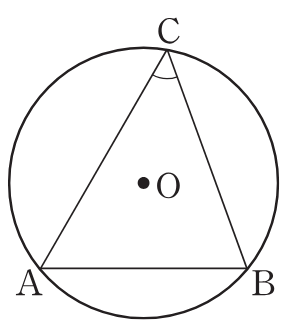
\includegraphics[width=68.5pt]{figures/fig-79-11-2.png}\end{minipage}\par
\begin{choicesii}{$50^\circ$}{$55^\circ$}{$60^\circ$}{$65^\circ$}{$70^\circ$}\end{choicesii}
